\documentclass[a4paper,12pt]{article}
\usepackage[left=1.5cm,right=1.5cm,
    top=1cm,bottom=1.5cm,bindingoffset=0cm]{geometry}

\usepackage[T1,T2A]{fontenc}
\usepackage[utf8]{inputenc}
\usepackage[english,russian,ukrainian]{babel}
\usepackage{tabularx}
\usepackage{amssymb}
\usepackage{color}
\usepackage{amsmath}
\usepackage{mathrsfs}
\usepackage{listings}
\lstset{language=Python, extendedchars=\true}
\usepackage{graphicx}
\graphicspath{ {./images/} }
%\usepackage{draftwatermark} не будет лезть на картинки
\usepackage[printwatermark]{xwatermark}%будет лезть на картинки
\usepackage{lipsum}
\usepackage{xcolor}
\usepackage{tikz}
%\newsavebox\mybox
%\savebox\mybox{\tikz[color=red,opacity=0.1]\node{AnMn.test};}
%\newwatermark*[allpages,angle=45,scale=11,xpos=-40, ypos=35]{\usebox\mybox}
\definecolor{lgreen}{rgb}{0.5,1,1}
\definecolor{n}{rgb}{1,0.5,0.5}
\definecolor{n1}{rgb}{1,1,0.5}
\definecolor{n3}{rgb}{1,0.7,0.9}
\usepackage{subcaption,floatrow,graphicx,calc}
\floatsetup{floatrowsep=qquad}



\begin{document}
\pagecolor{white}
\pagestyle{plain}
\begin{center}
   \begin{center} 
   \large{\textbf{Міністерство освіти і науки України} \par 
   \textbf{Національний технічний університет України}}\par
	“Київський політехнічний інститут”\par
	 Факультет електроніки\par
    	Кафедра мікроелектроніки\par
    \end{center}
    \vspace{4cm}
    
   	{\bfseries ЛАБОРАТОРНА РОБОТА № 1\par}
        \vspace{1cm}
        \large
        {
    	з курсу\par
    	«Теорія сигналів» \par
      	"Основи програмування мовою Python" \par  
	}
	\end{center}

       \vspace{7cm}
       \begin{tabularx}{\textwidth}{Xr}
        \flushright
           \begin{large} 
        Студента 3 курсу\par
 	групи ДП-81\par
	Фіцая Богдана\par
	 \end{large}
	\end{tabularx}
   
   \vfill
   \begin{center}
    {Київ} --- 2020
    \end{center}
%-----------------------------------------------------------------------------------------------------    
 \newpage   

\begin{center}
\textbf{Пункт 3}\par
\end{center}
Ознайомитися:\\
- з задаванням масиву, елементи якого є арифметичною послідовністю;\\
- з роботою функцій генерації випадкових чисел із заданими густинами розподілу імовірності. Ознайомитися з функцією побудови гістограм, побудувати гістограми випадкових чисел з різними розподілами густини ймовірності;\\

\begin{lstlisting}[language=Python]
import matplotlib.pyplot as plt
import matplotlib.mlab as mlab
import numpy as np
mas = [i for i in range(50)]
print(mas)

fig ,axs = plt.subplots(2,2)

a = np.random.standard_exponential(500)
b = np.random.standard_cauchy(100)
c = np.random.normal(size = 600)
d = np.random.laplace(size = 700)


axs[0,0].hist(a, bins=200)#Exponential distribution
axs[0,1].hist(b, bins=100)#Cauchy distribution
axs[1,0].hist(c, bins=200)#Normal distribution
axs[1,1].hist(d, bins=200)#Laplace distribution

plt.show()

\end{lstlisting}


\includegraphics[trim=3cm 0 0 -0.5cm, height = 16 cm, width =  19 cm]{gistogrammb.png}



\begin{center}
\textbf{Пункт 4}\par
\end{center}
Ознайомитися з написанням власних файлів-сценаріїв. У власному файлі-сценарії побудувати графік лінійної функції однієї змінної. Позначити вісі та заголовок графіку, нанести координатну сітку.\par
\begin{lstlisting}[language=Python]
import numpy as np
import matplotlib.pyplot as plt
from matplotlib import rc
rc('text', usetex=True)
rc('text.latex',unicode=True)
rc('text.latex',preamble='\usepackage[utf8]{inputenc}')
rc('text.latex',preamble='\usepackage[russian]{babel}')

x = np.linspace(3, 5, 10)
y = 1*x
plt.title(u"Линейная функция")
plt.xlabel('X')
plt.ylabel('Y')
plt.grid(True)
plt.plot(x, y, "r")
plt.show()
\end{lstlisting}
\begin{center}
\includegraphics[height = 12 cm,width=14 cm]{4f.png}
\end{center}
\vspace{1cm}\par



\begin{center}
\textbf{Пункт 5}\par
\end{center}
\textbf{5.1} Побудувати графіки синусоїд частот 1, 10, 50 Гц. Тривалість сигналів – 1 сек., частота дискретизації 256 Гц. Графіки будувати в одному вікні, але в різних осях. Амплітуди кожної синусоїди повинні бути випадковими числами.\par
\textbf{5.2} Виконати теж саме, але  задавати амплітуду кожної синусоїди з клавіатури.\par
\textbf{5.3} Підписати заголовок кожного графіку текстом, який буде містити значення частоти та амплітуди відповідної синусоїди.\par
\lstset{language=Python}          % Задаем язык исходного кода

\begin{lstlisting}[language=Python]
from numpy import array, arange, abs as np_abs

from math import sin, pi
import matplotlib.pyplot as plt
import matplotlib as mpl
import random

fr=1.
dfr = 256
dlinna = 256
ampl=random.uniform(1,10)
W=2.*pi*fr/dfr


plt.subplot(3,1,1) 
signal = array([ampl*sin(W*a) for a in range(dlinna)])
plt.plot(arange(dlinna)/float(dfr), signal, 'y')
plt.xlabel('Time, s')
plt.ylabel('Amplitude')
plt.title('Amplitude = '+  str(ampl)+' F = ' +  str(fr))
plt.grid(True)
plt.hold(True)

fr=10.
dfr = 256
dlinna = 256
ampl=random.uniform(1,10)
W=2.*pi*fr/dfr

plt.subplot(3,1,2) 
signal = array([ampl*sin(W*a) for a in range(dlinna)])
plt.plot(arange(dlinna)/float(dfr), signal, 'g')
plt.xlabel('Time, s')
plt.ylabel('Amplitude')
plt.title('Amplitude = '+  str(ampl)+' F = ' +  str(fr))
plt.grid(True)
plt.hold(True)

fr=50.
dfr = 256
dlinna = 256
ampl=random.uniform(1,10)
W=2.*pi*fr/dfr

plt.subplot(3,1,3) 
signal = array([ampl*sin(W*a) for a in range(dlinna)])
plt.plot(arange(dlinna)/float(dfr), signal, 'b')
plt.xlabel('Time, s')
plt.ylabel('Amplitude')
plt.title('Amplitude = '+  str(ampl)+' F = ' +  str(fr))
plt.grid(True)
plt.hold(True)
plt.show()
\end{lstlisting}
\begin{center}
\includegraphics[height = 11.5 cm,width=13 cm]{5f.png}
\end{center}
%-----------------------------------------------------------------------------------------------------    
\begin{center}
\textbf{Пункт 6}\par
\end{center}

\textbf{6.1} Побудувати одиночний прямокутний імпульс. Задати проміжок значень часу 10 секунд, частота дискретизації 256 Гц. Побудувати графік одиничного прямокутного імпульсу шириною 300 мс, з центром в момент часу 4 с.\par

\begin{lstlisting}[language=Python]
from numpy import array, arange, abs as np_abs
import matplotlib.pyplot as plt
from matplotlib import rc

rc('text', usetex=True)
rc('text.latex',unicode=True)
rc('text.latex',preamble='\usepackage[utf8]{inputenc}')
rc('text.latex',preamble='\usepackage[russian]{babel}')

fd = 256.
dt = 1./fd
Amp = 5.
b = 0.3
a = 4.0 - b/2
t_minimum = 0
t_maximum = 10.

def qwe(x):
    if x < a:
        return 0
    if x < a+b:
        return Amp
    return 0

x = [];
y = [];
t = t_minimum
while t<=t_maximum:
    x.append(t)
    y.append(qwe(t))
    t += dt

axes = plt.gca()
axes.set_xlim([-1,10])
axes.set_ylim([-1,8])
plt.plot(x, y, 'k')
plt.xlabel('Time, s')
plt.ylabel('Amplitude')
plt.title(u'Прямокутний iмпульс' )
plt.grid(True)

plt.show()

\end{lstlisting}
\begin{center}
\includegraphics[height = 11.5 cm,width=15 cm]{6.1f.png}
\end{center}

\textbf{6.2} Написати файл-сценарій для побудови графіку прямокутного імпульсу, тривалість та амплітуда якого буде задаватися з клавіатури. Розташування імпульсу задавати випадковим числом, але передбачити перевірку, чи не виходе імпульс за межі графіка.


\begin{lstlisting}[language=Python]
from numpy import array, arange, abs as np_abs
from math import sin, pi
import matplotlib.pyplot as plt
import matplotlib as mpl
import random
import numpy as np
from matplotlib import rc

rc('text', usetex=True)
rc('text.latex',unicode=True)
rc('text.latex',preamble='\usepackage[utf8]{inputenc}')
rc('text.latex',preamble='\usepackage[russian]{babel}')

def sqwave(p,X,T,aa,A,fd):
    x = []
    r = np.arange(p,X,1.0/fd)
    taue = aa+T
    x00 = r[(np.abs(r - aa)).argmin()]
    x01 = r[(np.abs(r - taue)).argmin()]
    if aa+T > X:
        return 1
    for i in r:
        if i >= x00 and i <= x01:
            x.append(A)
        else:
            x.append(0.0)
    return [r, x]

print('Input duration of impuls:')
duration = float(input())
print('Enter Amplitude:')
Amp = float(input())
a = sqwave(0, 10, duration, np.random.rand(1) * 10.0, Amp, 256.0)
while a == 1:
    a = sqwave(0, 10, duration, np.random.rand(1) * 10.0, Amp, 256.0)
plt.plot(a[0], a[1], 'm')
plt.title(u'Прямокутний iмпульс')
plt.ylabel(u'Амплiтуда')
plt.xlabel(u'Час, с')
plt.grid(True)
axes = plt.gca()
axes.set_xlim([-1,11])
axes.set_ylim([-1,Amp+2.0])
plt.show()

\end{lstlisting}
\begin{center}
\includegraphics[height = 12 cm,width=15 cm]{6.2.png}
\end{center}

\textbf{6.3} Побудувати послідовність прямокутних імпульсів для двох випадків: а) коли інтервали між імпульсами однакові, б) коли інтервали між імпульсами випадкові і задаються програмно.

\begin{lstlisting}[language=Python]
from numpy import array, arange, abs as np_abs
from math import sin, pi
import matplotlib.pyplot as plt
import matplotlib as mpl
import random
from matplotlib import rc

rc('text', usetex=True)
rc('text.latex',unicode=True)
rc('text.latex',preamble='\usepackage[utf8]{inputenc}')
rc('text.latex',preamble='\usepackage[russian]{babel}')

fd = 256.
t_minimum = -1.
t_maximum = 101.
delta_t = 1.0/fd;
print ('Амплитуда: ')
A = input()
print ('Ширина from 1 up to 10 : ')
b = input()
print ('Відстань між імпульсами: ')
a = input()
if b>10:
	print (u'Iмпульс за графiком!!!!!!!!!!')
	exit()
def qwe(x,imp_n,imp_d):
    if x < imp_n:
        return 0;
    if x < imp_n+imp_d:
        return A;
    return 0;



x = [];
y = [];
t = t_minimum;
while t<=t_maximum:
    k = t
    l = t + a + b
    m = t+a
    while k<=l:
        x.append(t);
        y.append(qwe(t,m,b));
        k += delta_t
        t += delta_t

plt.subplot(2,1,1)
plt.plot(x, y, 'k')
plt.title(u'Рандомна відстань')
plt.xlabel('Time, s')
plt.ylabel('Amplitude')
plt.grid(True)
axes = plt.gca()
axes.set_xlim([-1,101])
axes.set_ylim([-1,A+1])
plt.hold(True)


x1 = [];
y1 = [];
t = t_minimum;
while t<=t_maximum:
    k = t
    o = random.uniform(1,10)
    l = t + o + b
    m = t+o
    while k<=l:
        x1.append(t);
        y1.append(qwe(t,m,b));
        k += delta_t
        t += delta_t

plt.subplot(2,1,2)
plt.plot(x1, y1, 'm')
plt.title(u'Рандомна відстань')
plt.xlabel('Time, s')
plt.ylabel('Amplitude')
plt.grid(True)
axes = plt.gca()
axes.set_xlim([-1,101])
axes.set_ylim([-1,A+1])
plt.hold(True)
plt.show()
\end{lstlisting}
\begin{center}
\includegraphics[height = 13 cm,width=16 cm]{6.3f.png}
\end{center}
%________________________________________________



\begin{center}
\textbf{Пункт 7}\par
\end{center}
Зберегти дані розрахунку функції в файл. Прочитати їх із файлу в іншому сценарії, побудувати графік функції.\par

\begin{lstlisting}[language=Python]
import numpy as np
import matplotlib.pyplot as plt
from matplotlib import rc

rc('text', usetex=True)
rc('text.latex',unicode=True)
rc('text.latex',preamble='\usepackage[utf8]{inputenc}')
rc('text.latex',preamble='\usepackage[russian]{babel}')

ex_2 = np.load('SAVE.npz')
ex_2.files
x = ex_2['arr_0']
y = ex_2['arr_1']
Amplitude = ex_2['arr_2']

plt.plot(x, y, Amplitude, 'k')
plt.title(u'Прямокутний iмпульс прочитаний з файлу SAVE.npz')
plt.xlabel('Time, s')
plt.ylabel('Amplitude')
plt.grid(True)
axes = plt.gca()
axes.set_xlim([-1,11])
axes.set_ylim([-1,Amplitude+1])
plt.show()
\end{lstlisting}
%\begin{center}
%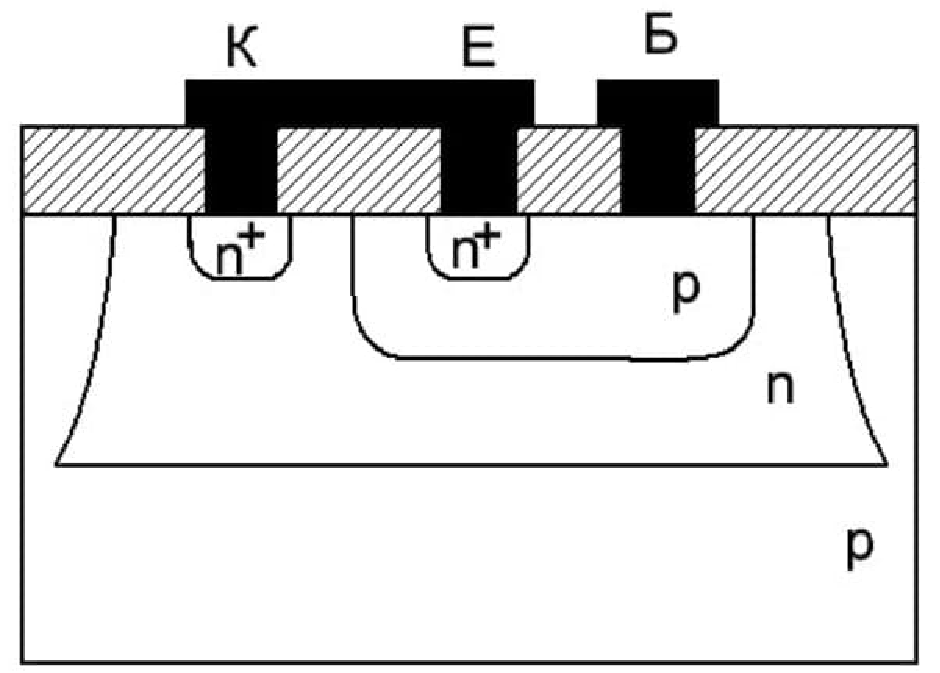
\includegraphics[height = 12 cm,width=15 cm]{7.png}

\begin{center}
{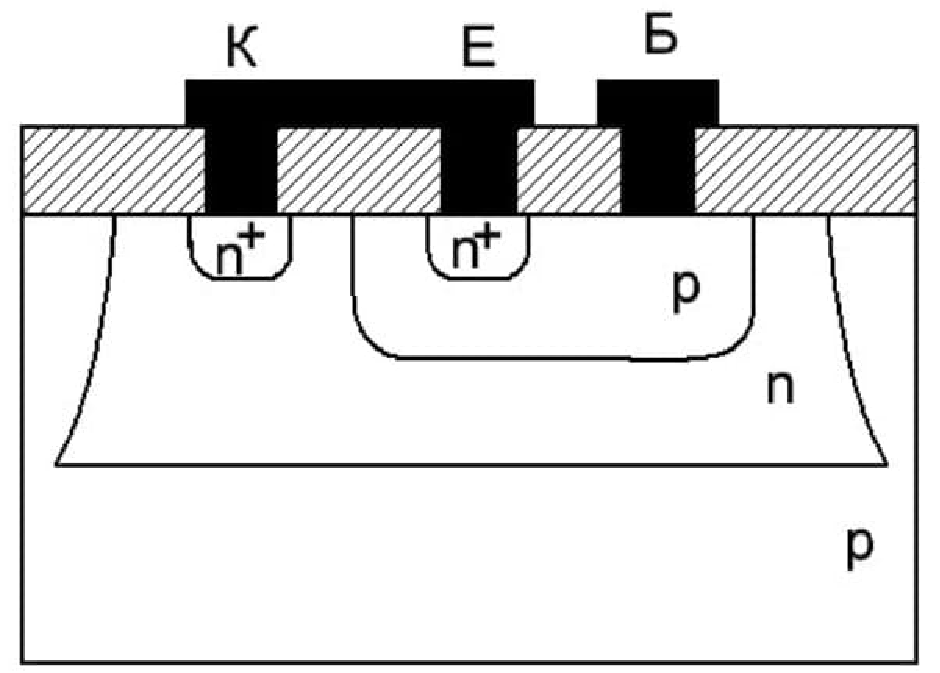
\includegraphics[height = 10 cm,width=13 cm]{7.png} }\\
\end{center}

\begin{center}
\textbf{Пункт 8}\par
\end{center}
 Побудувати власний файл-функцію для побудови графіка синусоїдального сигналу із заданою частотою, амплітудою та тривалістю для частоти дискретизації 256 Гц. В якості вихідного параметру функції вивести середнє значення синусоїди. \par

\begin{lstlisting}[language=Python]
from numpy import array, arange, abs as np_abs
from math import sin, pi
import matplotlib.pyplot as plt
import random
from matplotlib import rc
rc('text', usetex=True)
rc('text.latex',unicode=True)
rc('text.latex',preamble='\usepackage[utf8]{inputenc}')
rc('text.latex',preamble='\usepackage[russian]{babel}')

def qwe():
f=1.
	fd = 256
	n = 256
	W=(2.*pi*f/fd)
	Amplitude=random.uniform(1,10)

	signal = array([Amplitude*sin(W*q) for q in range(n)])
	plt.plot(arange(n)/float(fd), signal, 'b')
	plt.xlabel('Time, s')
	plt.ylabel('Amplitude = '+  str(Amplitude))
	plt.title(u'Синусоїдальний сигнал, з частотою  ' +  str((f)))
	plt.grid(True)
	plt.hold(True)
	plt.show()
	return A*0.637

print (qwe())
\end{lstlisting}
\begin{center}
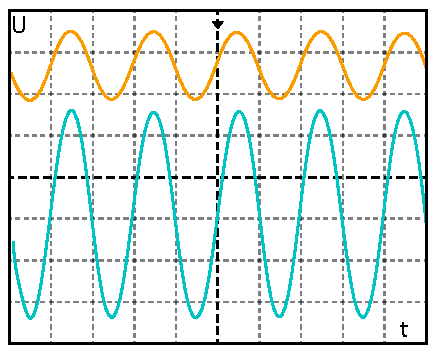
\includegraphics[height = 12 cm, width=18 cm]{8.png}\par
\vspace{1cm}
\end{center}
Відповідь: cереднє значення синусоїди = 2.18





\end{document}